Anteriormente, en la imagen \ref{fig:docker-interface} se muestra cómo el
motor Docker interactúa con el kernel de Linux para proveer aislamiento. Entre
otras librerías, Docker usa en particular los \textit{cgroups} 
\autocite{Cgroups2021} y los \textit{namespaces} de Linux \autocite{LinuxNamespaces2021}.

Sendas funcionalidades del kernel ofrecen una gran capa de seguridad y aislamiento
de procesos de forma nativa en todas las máquinas Linux, y Docker aprovecha esa
infraestructura para proteger los contenedores a un nivel muy bajo: a nivel de
kernel.

Este planteamiento ya augura un buen presagio en tanto que no se usan aplicaciones
externas o librerías de terceros para el aislamiento y protección de capas sino
que se usa una arquitectura a bajo nivel ampliamente depurada y probada como es
el kernel de Linux. Además, esto permite también una gran portabilidad, ya que
el ``único requisito'' para ejecutar Docker sería contar con un kernel de 
Linux.

A la hora de hablar o revisar la seguridad de Docker, existen cuatro áreas
primordiales en las que indagar \autocite{DockerSecurity2021}:

\begin{itemize}
  \item La seguridad intrínseca del kernel así como su soporte para \textit{namespaces}
        y \textit{cgroups}.
  \item La superficie de ataque sobre el servicio de Docker en sí.
  \item Lagunas en las configuraciones de un contenedor o bien por defecto o bien
        introducidas por el usuario.
  \item Las características de seguridad del kernel y su interacción con Docker.
\end{itemize}

\subsubsection*{Linux kernel \textit{namespaces}}
A nivel de funcionamiento, Docker es similar a los contenedores LXC y comparten
los mismos mecanismos de seguridad. Por ende, cuando se crea un contenedor con el comando
\lstinline[style=bash]!docker run! internamente se están creando un conjunto
de \textit{namespaces} y \textit{cgroups} para el contenedor.

El primero ofrece la primera y mayor forma de aislamiento -- un proceso que se
ejecuta dentro de un \textit{namespace} es incapaz de ver (y mucho menos afectar)
a otros procesos en ejecución en otro contenedor o en la máquina anfitriona.

Esto llega al nivel de que cada contenedor tiene su propia pila de protocolos de
red, lo cual implica que un contenedor nunca tendrá acceso privilegiado a \textit{sockets}
o interfaces de otro contenedor o del sistema anfitrión. Sin embargo, si se configura
correctamente un sistema anfitrión las comunicaciones entre contenedores pueden
existir perfectamente, a través de la misma interfaz de red. Si por el contrario se
expone el puerto del contenedor entonces otros equipos podrán enviarle mensajes
o \textit{pings} al contenedor, paquetes TCP/UDP y establecer distintos tipos de
conexiones. Sin embargo, se pueden restringir si es necesario: a fin de cuentas,
la interfaz por defecto que usan los contenedores es la tipo puente, que implica
que en apariencia son equipos conectados a un \textit{switch}.

Por otra parte, los \textit{namespaces} de Linux tienen la ventaja de que son
prestaciones probadas y testeadas a lo largo del tiempo, introducidas en el año
2008 en la versión \texttt{2.6.15}. Además, su diseño y arquitectura
se basa en un intento de mejora sustancial de OpenVZ \autocite{OpenVZ2021},
desarrollado en 2005.

En un estudio realizado en el año 2018 \autocite{sunSecurityNamespaceMaking2018}, se
detectaron ciertos problemas residentes en el kernel que impedían a los contenedores
hacer uso de características avanzadas de seguridad del kernel: no se pueden
aplicar políticas para comprobar la integridad, regular la ejecución de código,
control de acceso, etc. que permiten prevenir problemas de seguridad referentes
a la aplicación. Ante el intento de añadir nuevas opciones al kernel que permitan
el acceso a dichos recursos, se descartaron debido a ser solución \textit{ad-hoc}
que suponían muchas veces una brecha de seguridad más allá de una opción
real.

Sin embargo, en dicho estudio se proponen los \textit{security namespaces}, una
característica del kernel que permitiría la ejecución de contenedores con la
totalidad de las prestaciones disponibles produciendo una latencia menor al
$0.7\%$ en las llamadas al sistema.

Esta característica ha seguido evolucionando hasta nuestros días en la forma de
los \textit{user namespaces}, que son los usados e implementados actualmente
por Docker. Un problema común del usuario \texttt{root} en Linux no es que sea
necesariamente el administrador sino las posibilidades que tiene (en particular,
las Linux kernel \textit{capabilites} \autocite{CapabilitiesLinuxManual}):
estas capacidades se pueden otorgar o bien mediante un escalador de privilegios
(por ejemplo, usar el comando \texttt{sudo}) o mediante el ajuste de permisos,
como el \texttt{SUID} o un cambio de \textit{namespace}. Esto se aprovecha por
el motor Docker para definir qué posibilidades tiene un contenedor, que pueden
ser añadidas o restringidas por el usuario.

El problema es cuando un usuario define un contenedor que requiere de más
capacidades de las que él mismo tiene. Por defecto, los contenedores se
ejecutan siempre como \texttt{root}, por lo que la situación anterior es
perfectamente posible, y conlleva posibles abusos en forma
de fallo de seguridad.

Con el uso de los \textit{user namespaces} este problema se puede abordar
fácilmente: un \textit{namespace} es a fin de cuentas un ``mapa'' en donde
un UID y GID virtuales se mapean con los UID/GID reales y se exponen
en la ruta \texttt{/proc} \autocite{blogEvolvingContainerSecurity2021}. El mapeo
presenta la siguiente forma (figura \ref{fig:ns-mapping}):

\begin{figure}[H]
  \centering
  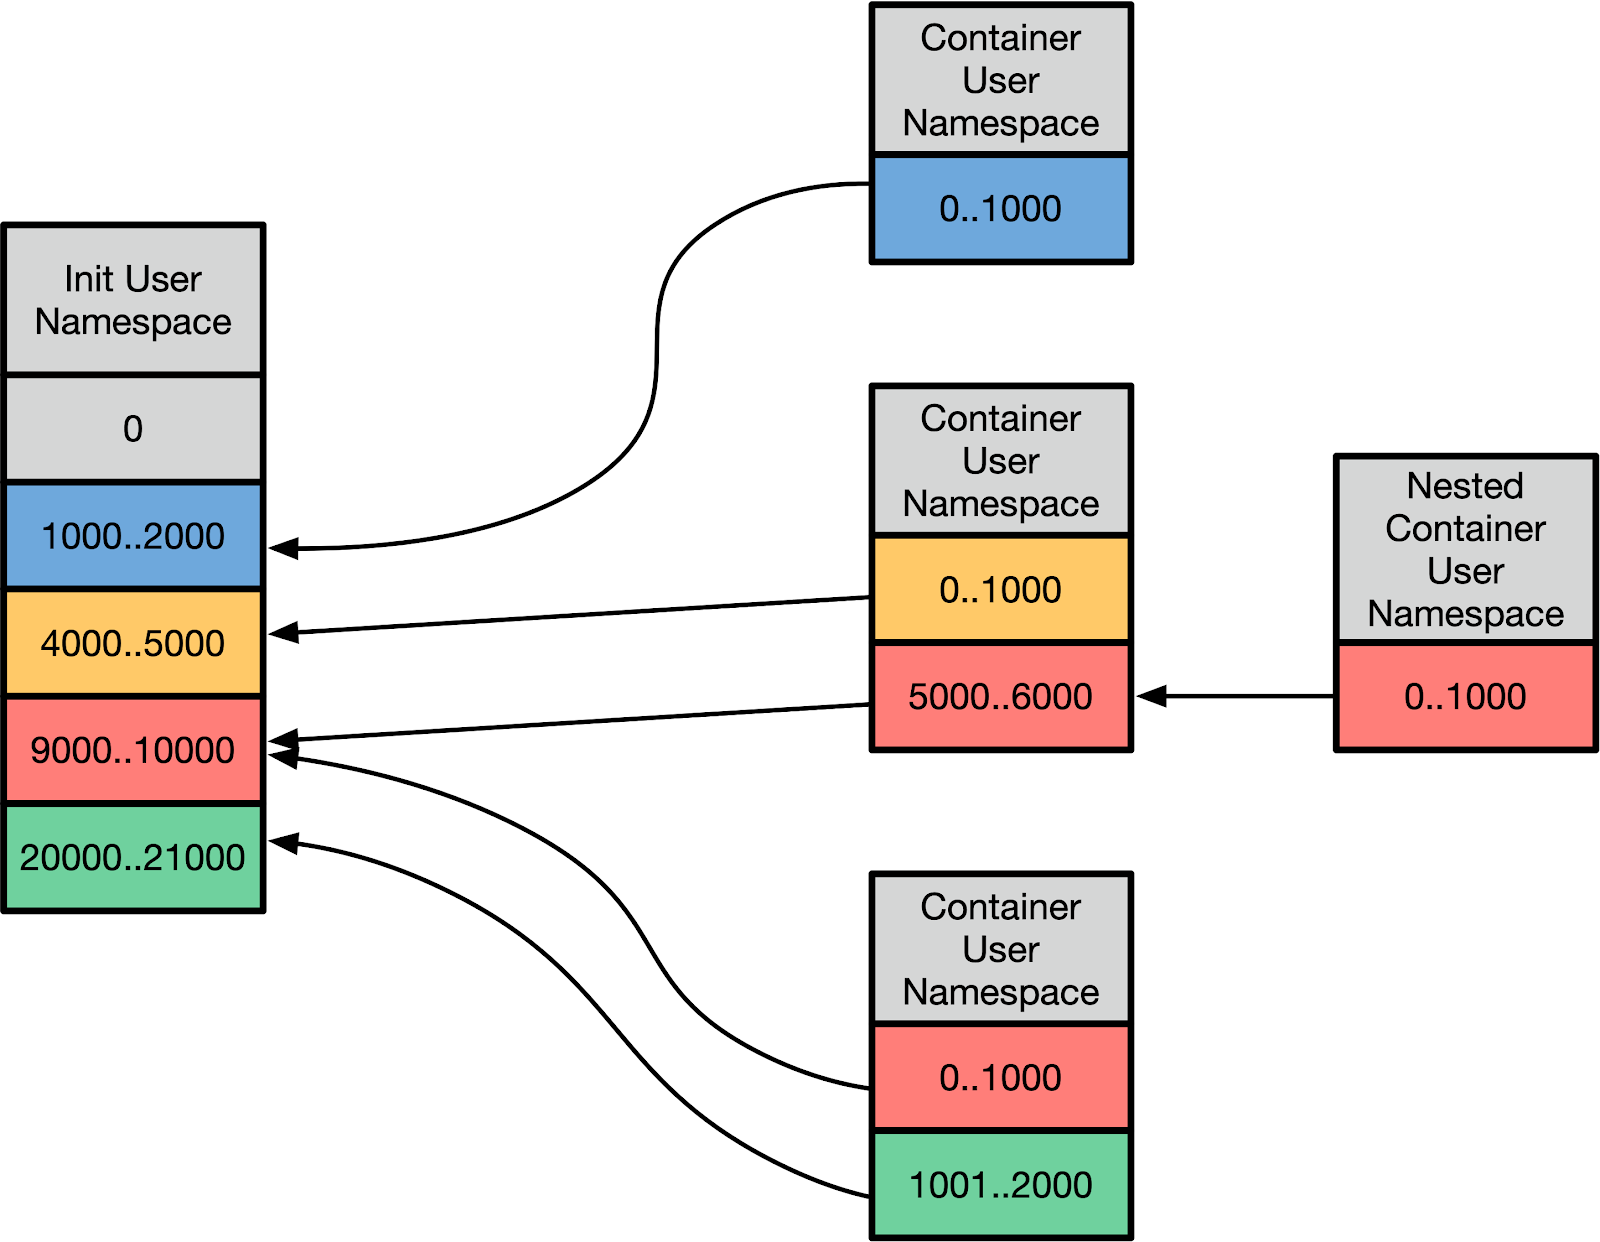
\includegraphics[width=\linewidth]{pictures/ns_mapping.png}
  \caption{Mapeo de los UID del \textit{namespace} del contenedor al \textit{namespace} del sistema \autocite{blogEvolvingContainerSecurity2021}.}
  \label{fig:ns-mapping}
\end{figure}

¿Por qué es potente esta característica del sistema?:

\begin{itemize}
  \item Permite, por una parte, definir ciertos UIDs únicamente dentro del
        contenedor. De esta forma, si un UID no está relacionado con un UID real
        del equipo anfitrión, al intentar examinar un fichero con dicho UID
        aparecerá un error del tipo \texttt{overflowuid} en los ficheros
        de \texttt{/proc} \autocite{DocumentationProcSys}.
  \item Desde el punto de vista de un \textit{namespace} de usuario el contenedor 
        se ejecuta con UID $0$ cuando en realidad está usando un rango de valores
        mapeados en dicho \textit{namespace}.
  \item Los subsistemas Linux pueden ejecutar la función ``\lstinline[style=C]!ns_capable!''
        (que permite definir si una tarea tiene en realidad mayores capacidades) usando un \textit{namespace} específico de un recurso. De esta forma,
        los procesos pueden realizar acciones ``privilegiadas'' sin tener en
        realidad privilegios sobre el sistema anfitrión.
\end{itemize}

En la actualidad, el servicio Docker inicia los contenedores siempre con las
capacidades mínimas posibles \autocite{DockerSecurity2021}: por ejemplo,
servidores web que únicamente necesitan exponer un puerto protegido ($< 1024$)
se le garantiza el permiso \texttt{net\_bind\_service} en lugar de ejecutarse
como administrador.

Esto permite que diversos procesos que siempre se ejecutan como administrador
(SSH, cron, módulos del kernel, \dots) usen un usuario con menos privilegios
y se les garantice únicamente acceso a las características que necesitan. Algunas
operaciones además son directamente gestionadas por Docker en lugar de por
las aplicaciones que se ejecutan:

\begin{itemize}
  \item El acceso mediante SSH se realiza mediante un único servidor gestionado por Docker.
  \item Los procesos \texttt{cron} se ejecutan como usuario estándar, cuando es posible.
  \item La gestión de \textit{logs} se delega a Docker u otro servicio.
  \item La gestión del \textit{hardware} es irrelevante, lo que se traduce en que
        instrucciones como \texttt{udevd} nunca serán necesarias.
  \item La gestión de las redes sucede fuera de los contenedores, lo cual implica
        que un contenedor nunca tendrá que ejecutar tareas con \texttt{ifconfig},
        \texttt{route} o \texttt{ip}.
\end{itemize}

La implicación directa es que los contenedores no necesitan permisos de administrador
reales (al menos, no todos) y se restringen las posibilidades del mismo. Por ende,
se pueden aplicar algunas medidas de seguridad que impliquen denegar todas las 
operaciones de montaje, impedir el acceso a sockets, prohibir ciertas operaciones
sobre discos (particionado, cambiar permisos, etc.), denegar la carga de módulos
del kernel y demás.

Así, si un intruso es capaz de acceder a un contenedor y escalar privilegios hasta
ser \texttt{root}, el daño que podrá hacer sobre el sistema estará limitado. Pero
esto siempre ha de ir acompañado de una gestión competente: cuando se crea un
contenedor, lo ideal sería quitar todas aquellas capacidades del contenedor que
no sean necesarias o no se vayan a usar.

\subsubsection*{Linux \textit{control groups}}
Los grupos de control de Linux no son necesariamente una característica de seguridad
sino de control y regulación de acceso a los recursos. En el estudio mencionado
anteriormente (\autocite{sunSecurityNamespaceMaking2018}) uno de los problemas
que se vieron en comparación con las máquinas virtuales era la restricción del
acceso a los recursos y la limitación de ciertas acciones.

Durante bastante tiempo los contenedores Docker no contaban con una limitación en
la cantidad de recursos disponibles hasta que se adaptó el motor de ejecución
para trabajar con los \textit{cgroups}, que existen en Linux desde el 2006
(versión \texttt{2.6.24} \autocite{DockerSecurity2021}).

Esta característica se incluye en el apartado de seguridad porque permite
proteger a un contenedor de ataques de denegación de servicio, ``molestar'' a otro
contenedor, etc.

\subsubsection*{Ataque al servicio de Docker}
La ejecución de contenedores implica el uso del servicio de Docker para ello. Si
no se ha optado por el modo ``sin privilegios'', dicho servicio se ejecutará siempre
como \texttt{root}, por lo que será uno de los elementos más atacados
y vulnerables que existan.

En general, sobre el servicio Docker no se pueden tomar muchas acciones en lo
referente a privilegios o código fuente pero sí se pueden aplicar ciertas restricciones
sobre el uso. Lo primero es restringir qué usuarios pueden interactuar con el
servicio de Docker, ya que es una implicación directa de seguridad. En Docker,
se puede hacer \textit{bind mounts} del directorio raíz del sistema (\texttt{/})
dentro de un directorio \texttt{/host} en el contenedor. Desde allí, se puede
acceder a cualquier fichero, directorio o dispositivo sin restricciones ni
limitaciones.

Es por este motivo por el que Docker CLI utiliza una API REST contra un socket
UNIX en lugar de usar la dirección \texttt{127.0.0.1}, ya que permite ajustar
los permisos del socket usando el sistema de permisos de Linux. Bajo esta
premisa, si se decidiese crear un contenedor que expusiera una API REST bajo
HTTP habría que dedicar especial atención a qué ficheros se puede acceder y
controlar todavía más los parámetros que se reciben. Inclusive aunque se restrinja
el acceso a la API únicamente a la red local mediante el uso de \textit{firewalls},
otros contenedores podrían comprometer el sistema. Por ello, es obligatorio
proteger los \textit{endpoints} usando HTTPS y certificados digitales, y altamente
recomendable que solo sea accesible a través de una VPN.

Por otra parte, el servicio Docker es potencialmente vulnerable a otras entradas como
la carga de una imagen desde el disco con \lstinline[style=bash]!docker load!
o desde la red con \lstinline[style=bash]!docker pull!. Por ello, el primer paso
desde la versión \texttt{1.10.0} de Docker es la de crear una jaula \texttt{chroot}
en donde desempaquetar la imagen y preparar el entorno. Para evitar estos problemas
se puede configurar el servidor Docker para que únicamente trabaje con imágenes
firmadas -- DCT (\textit{Docker Content Trust}).

Esta característica es nativa al servicio de Docker y se puede usar
directamente desde Docker CLI. Mediante esta herramienta, un usuario que
publique una imagen podrá firmarla y darle la seguridad a los clientes
de que se está usando una imagen oficial. Las claves de firma se disgregan
en tres tipos de claves:

\begin{itemize}
  \item Claves offline, para la firma inicial de la imagen asociada a un usuario.
  \item Clave de etiquetado (\textit{tag key}), asociada a un repositorio de imágenes.
  \item Clave de tiempo (\textit{timestamp key}), asociada a un repositorio y creada
        por Docker.
\end{itemize}

Todas las claves se generan a raíz de la clave offline, también conocida como
``\textit{root key}'' (figura \ref{fig:keys}):

\begin{figure}[H]
  \centering
  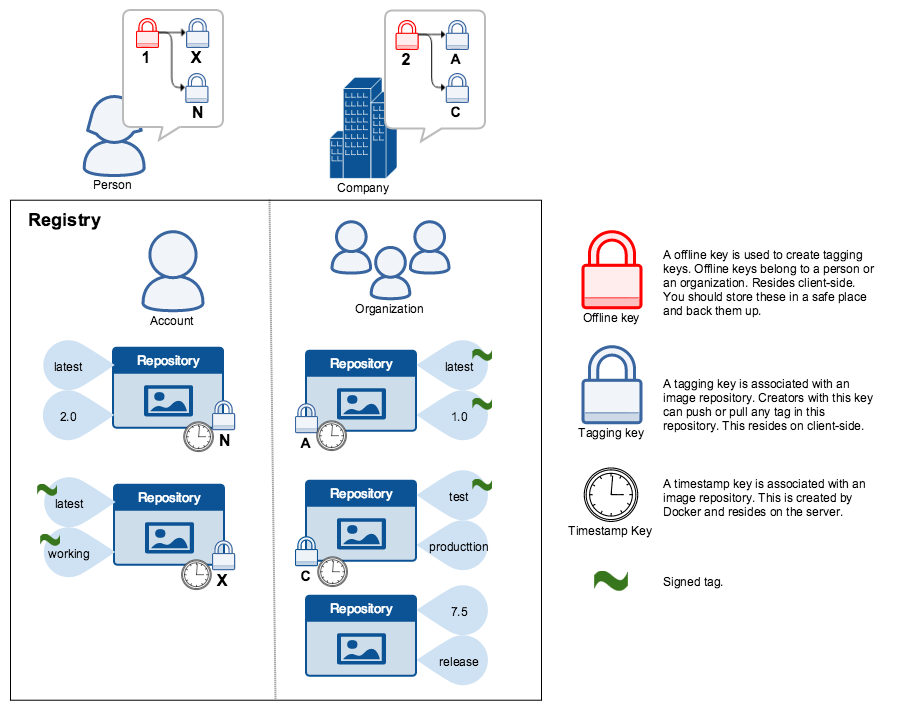
\includegraphics[width=\linewidth]{pictures/trust_components.png}
  \caption{Distribución de las claves para la firma de imágenes en Docker \autocite{ContentTrustDocker2021}.}
  \label{fig:keys}
\end{figure}

\subsubsection*{Mayor protección de Docker}
Una de las características fundamentales de que se ejecute sobre el kernel de Linux
es que Docker está directamente integrado con otras herramientas de seguridad.

Aunque el motor Docker deshabilite ciertas posibilidades sobre los contenedores
esto no implica que otros sistemas no se puedan usar en conjunto. Por ejemplo:

\begin{itemize}
  \item Se puede ejecutar un kernel con GRSEC \autocite{Grsecurity} y PAX \autocite{PaX2019}
        para añadir opciones de seguridad tanto en la compilación como en tiempo
        de ejecución. Por otra parte, mediante el uso de técnicas de seguridad como
        la aleatorización de direcciones se mitigan muchas vulnerabilidades
        del sistema. Lo interesante es que no es necesaria ninguna interacción
        por parte de Docker ya que son características que se aplican a lo largo
        de todo el sistema.
  \item Si la aplicación viene con un modelo de seguridad que use AppArmor o SELinux
        se puede integrar directamente dentro de Docker, sin necesidad de hacer
        ningún cambio. Esto otorgará una capa extra de seguridad que se complementa
        con la restricción de las capacidades del contenedor.
\end{itemize}

En principio, cualquier herramienta externa se podría usar dentro de un contenedor
Docker para proteger el acceso y añadir más capas de seguridad. Esto se hace
principalmente sobre sistemas de ficheros en red o compartidos con otros
contenedores, donde la seguridad es crítica.